\section{Methods and Hyperparameters} \label{app:methods}

\subsection{Point Cloud Encoder} \label{app:pc_encoder}
In this section, we provide additional details on the point cloud encoders used in our comparisons.
\paragraph{PSTNet.}
We closely follow the method proposed in \citep{fan2021pstnet} and use the official implementation and architecture from \url{https://github.com/hehefan/Point-Spatio-Temporal-Convolution}. The spatial kernel radius is adapted to $0.1$ to match our task normalization, while all other architectural components and hyperparameters are kept unchanged.

\paragraph{GNN Encoder.}
At each timestep, we perform \gls{fps} to select $52$ center points per point cloud in the sequence. For each center point, we connect its $16$ nearest neighbors and apply a PointNet layer~\citep{qi2016pointnet} to each resulting patch, yielding an embedding of dimension $32$. We concatenate a Fourier encoding of the corresponding timestep to this embedding.

The resulting spatio-temporal tokens are then assembled into a graph: within each timestep, every node is connected to its $4$ nearest neighbors. In addition, each node is connected to its $2$ nearest neighbors in the subsequent timestep and to its single nearest neighbor in the following timestep. This construction yields a spatio-temporal graph encoding the complete point cloud sequence.

The graph is processed using a message-passing graph neural network~\citep{sanchezgonzalez2020learning} without global features, consisting of $5$ layers with a latent dimension of $128$. Finally, an attention-based readout module is applied to obtain a single output token.

\subsection{Test-Time Optimization}
\label{app:tto}
Test-Time Optimization represents the classical system identification approach, in which the unknown physical parameters are recovered by inverting a differentiable simulator on the observed data. We use the trained \textit{Oracle} model as the simulator, as it receives the physical parameters $\rho$ directly as input. We optimize the parameters in the same normalized space in which the \textit{Oracle} model receives them, without constraining them to the training range, and initialize them with the mean parameters of the training set.

\paragraph{Objective.}
In each optimization step, the \textit{Oracle} model predicts the mesh trajectories of all context trajectories given the current parameter estimate $\hat{\rho}$. We compare each predicted mesh with the observed point cloud of the same time step. Let $\mathcal{P}_t$ denote the observed point cloud with $N$ points at time step $t$, and $\mathcal{F}_t$ the set of triangles of the predicted meshes, including both the deformable object and the collider. The point-to-mesh distance assigns each observed point to its closest triangle and computes the squared distance to the closest point on that triangle as
\begin{equation*}
    \mathcal{L}_{\text{p2m}}(t) = \frac{1}{N} \sum_{\mathbf{p} \in \mathcal{P}_t} \min_{f \in \mathcal{F}_t} d(\mathbf{p}, f)^2 ,
\end{equation*}
where $d(\mathbf{p}, f)$ denotes the Euclidean distance between the point $\mathbf{p}$ and the triangle $f$.
This term only requires every observed point to lie close to the predicted surface, but does not penalize predicted surface regions that are not supported by any observation. We therefore optionally add a reverse mesh-to-point term, which computes the squared distance from the centroid $\mathbf{c}_f$ of each triangle to its nearest observed point, weighted by the triangle area $a_f$, as
\begin{equation*}
    \mathcal{L}_{\text{m2p}}(t) = \frac{\sum_{f \in \mathcal{F}_t} a_f \min_{\mathbf{p} \in \mathcal{P}_t} \| \mathbf{c}_f - \mathbf{p} \|^2}{\sum_{f \in \mathcal{F}_t} a_f} .
\end{equation*}
The total objective averages both terms over all time steps and all $C$ context trajectories,
\begin{equation*}
    \mathcal{L}(\hat{\rho}) = \frac 1 {TC} \sum_{c=1}^{C} \sum_{t=1}^{T} \Bigl( \mathcal{L}_{\text{p2m}}^{(c)}(t) + \lambda \, \mathcal{L}_{\text{m2p}}^{(c)}(t) \Bigr) ,
\end{equation*}
with a weight $\lambda$ for the reverse term. We minimize $\mathcal{L}$ with respect to $\hat{\rho}$ using Adam~\citep{kingma2014adam} and a step-wise learning rate decay. After the optimization, the \textit{Oracle} model predicts the target trajectory using the optimized parameters. The reverse term is necessary for \texttt{Deforming Block}, where the optimization does not converge to meaningful parameters without it, and we disable it for all other environments. Table~\ref{tab:tto_hparams} lists the hyperparameters, which we tuned per environment. For the real-world recordings, we use the same hyperparameters as for the simulated \texttt{Trampoline} environment.

\paragraph{Context size.}
Backpropagating through full rollouts of multiple context trajectories is memory intensive, so the number of context trajectories is limited by GPU memory for some environments. Additionally, we found that more context trajectories do not consistently improve the result of Test-Time Optimization. We therefore report the best result across the context sizes we could evaluate, which favors this baseline compared to the fixed context size of $8$ trajectories used for all other methods.

\begin{table}[t]
    \centering
    \caption{Hyperparameters of Test-Time Optimization. The learning rate is multiplied by the decay factor after every decay interval.}
    \label{tab:tto_hparams}
    \begin{tabular}{lcccc}
    \toprule
     & \shortstack{\texttt{Deforming}\\\texttt{Block}} & \shortstack{\texttt{Sheet}\\\texttt{Deformation}} & \shortstack{\texttt{Bending}\\\texttt{Beam}} & \texttt{Trampoline} \\
    \midrule
    Learning rate & $0.03$ & $0.03$ & $0.015$ & $0.06$ \\
    Optimization steps & $50$ & $200$ & $200$ & $300$ \\
    Decay interval (steps) & $25$ & $100$ & $100$ & $100$ \\
    Decay factor & $0.5$ & $0.25$ & $0.25$ & $0.25$ \\
    Reverse term weight $\lambda$ & $1.0$ & $0$ & $0$ & $0$ \\
    \bottomrule
    \end{tabular}
\end{table}

\subsection{Mesh Encoder and Simulator}
\paragraph{Mango Mesh Encoder.}
We closely follow the architecture of \citep{dahlinger2025mango} and apply a one-dimensional convolutional neural network to each node along the temporal dimension. The mesh structure provides consistent point correspondences over time, enabling this temporal processing. Node features are then aggregated using a Deep Set architecture \citep{cai2023deepset} to produce a permutation-invariant representation of the mesh. We use the official implementation, available at \url{https://github.com/ALRhub/mango}.


\paragraph{Mango Simulator.}\label{app:mango}
We closely follow the implementation from~\citep{dahlinger2025mango}, using the official code available at \url{https://github.com/ALRhub/mango}. Rather than maintaining separate graphs per timestep, \gls{mango} represents the trajectory as a single static graph $\mathcal{G} = (\mathcal{V}, \mathcal{E})$ with temporally indexed node and edge feature tensors $\mathbf{m}_v \in \mathbb{R}^{T \times |\mathcal{V}| \times d_\text{node}}$ and $\mathbf{m}_e \in \mathbb{R}^{T \times |\mathcal{E}| \times d_\text{edge}}$. The initial node features and trajectory-level conditioning variables, such as latent physical parameters, are broadcast across all time steps and augmented with a learned time embedding per timestep. Edge features are constructed from relative nodal positions. Both are then linearly projected into a latent dimension to obtain the initial feature tensors $\mathbf{m}_v^0$ and $\mathbf{m}_e^0$.
Spatial reasoning within each time step is performed via a message passing \gls{gnn} layer, which updates node and edge features based on local neighborhood interactions as
\begin{equation*}
    \mathbf m_e^{k+1} = f_\mathcal{E}^k(\mathbf m_e ^k, \mathbf m_v ^k, \mathbf m_w ^k)\text{, with } e=(v, w), \qquad \tilde {\mathbf m}_v^{k+1} = f_\mathcal{V}^k(\mathbf m_v ^k, \bigoplus_{e \in \mathcal{E}_v} \mathbf m_e ^{k+1}).
\end{equation*}
Here, $\mathcal{E}_v \subseteq \mathcal{E}$ denotes the edges incident to node $v$, and $\bigoplus$ is a permutation-invariant aggregation. The functions $f_\mathcal{E}^k$ and $f_\mathcal{V}^k$ are learned \glspl{mlp}.
The resulting node features $\tilde{\mathbf{m}}_v^{k+1}$ are then processed independently over time by a 1D residual \gls{cnn} to obtain $\mathbf{m}_v^{k+1}$. After $K$ rounds of spatial message passing interleaved with temporal \gls{cnn} processing, the model is trained by summing per-timestep \gls{mse} losses against ground truth mesh states over the full rollout.

\subsection{Parameters and Runtime}
\label{sec:runtime}
\gls{peach} has a total of $3.96$M parameters, of which $3.01$M belong to the \gls{mango} simulator and $0.96$M to the point cloud encoder and auxiliary loss heads.

We report inference timings on an NVIDIA RTX~5090 for the \texttt{Trampoline} environment, using $N=1024$ points per frame and every second time step of the trajectory unless stated otherwise. Inference consists of two stages. First, the encoder maps the context point cloud sequences to the aggregated latent material description. Second, the simulator predicts the full trajectory from the initial mesh and the latent description.

\paragraph{Encoding.}
Figure~\ref{fig:encoding_scaling} shows how the encoding time depends on the context size $C$, the number of points per frame $N$, and the number of frames per trajectory $T$. The encoding time grows with the context size from $73$\,ms for a single context trajectory to $229$\,ms for eight. For all point counts, we observe a step between $C=2$ and $C=3$, which we attribute to implementation effects of the batched GPU computation, such as a change in kernel selection for larger batches, rather than to the method itself. Doubling the number of points or the number of frames increases the encoding time by a factor between $1.6$ and $1.9$. This is consistent with the linear dependence on the total number of space-time points $N \cdot T$ of farthest point sampling and patch grouping.

\begin{figure}[t]
    \centering
    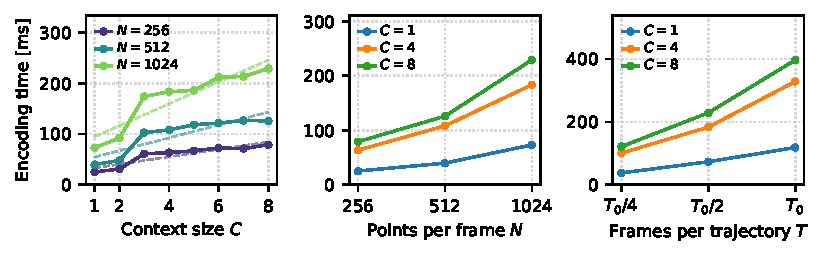
\includegraphics[width=\textwidth]{figures/encoding_scaling.pdf}
    \caption{Encoding time of \gls{peach} on the \texttt{Trampoline} environment. \textbf{Left.} Encoding time over the context size $C$ for different numbers of points per frame $N$, with linear fits shown as dashed lines. \textbf{Center.} Encoding time over the number of points per frame. \textbf{Right.} Encoding time over the number of frames per trajectory, where $T_0$ denotes the full trajectory length.}
    \label{fig:encoding_scaling}
\end{figure}

\paragraph{Simulation.}
The simulation rollout takes approximately $352$\,ms regardless of the context size, as it operates solely on the aggregated latent code. A complete prediction therefore takes between $0.4$ and $0.6$\,s, depending on the context size.

\paragraph{Comparison.}
Figure~\ref{fig:runtime_comparison} compares the inference time of \gls{peach} with \textit{Test-Time Optimization} and the \gls{fem} simulator used to generate the training data. \textit{Test-Time Optimization} requires $82$\,s to adapt to a task and predict its trajectory, as each of its optimization steps involves a full forward and backward pass through the simulator for all context trajectories. \gls{peach} replaces this iterative optimization with a single forward pass and is thus about $140$ times faster. A single \gls{fem} rollout requires $4$ minutes on an AMD EPYC 74F3 24-Core Processor, even with known material parameters. Identifying unknown parameters with the \gls{fem} simulator would require many such rollouts and thus take considerably longer.

\begin{figure}[t]
    \centering
    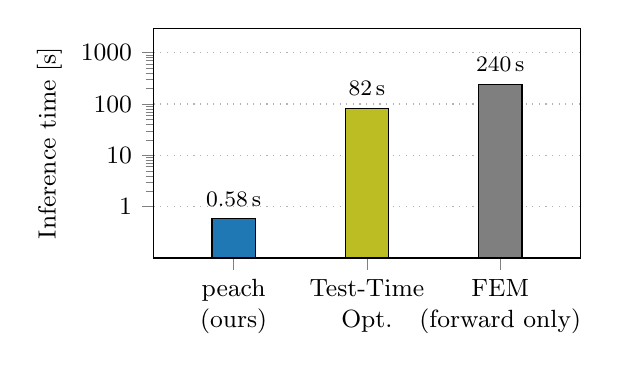
\begin{tikzpicture}
\definecolor{tabblue}{RGB}{31,119,180}
\definecolor{tabolive}{RGB}{188,189,34}
\definecolor{tabgray}{RGB}{127,127,127}

\begin{semilogyaxis}[
  width=7cm,
  height=4.5cm,
  ybar,
  bar width=0.55cm,
  % all bars centered on their own x position (no grouping offset)
  bar shift=0pt,
  % bars start at the lower axis limit instead of at y=1
  log origin=infty,
  ymin=0.1, ymax=3000,
  ytick={1,10,100,1000},
  yticklabels={1,10,100,1000},
  ylabel={Inference time [s]},
  symbolic x coords={PEACH,TTO,FEM},
  xtick={PEACH,TTO,FEM},
  xticklabels={{\gls{peach}\\(ours)}, {Test-Time\\Opt.}, {FEM\\(forward only)}},
  x tick label style={font=\small, align=center},
  enlarge x limits=0.3,
  ymajorgrids,
  grid style={dotted, gray!60},
  tick align=outside,
  ytick pos=left,
  xtick pos=bottom,
  tick label style={font=\small},
  label style={font=\small},
  nodes near coords,
  point meta=explicit symbolic,
  every node near coord/.append style={font=\footnotesize, yshift=1pt},
]
\addplot[fill=tabblue, draw=black, line width=0.5pt]
  coordinates {(PEACH,0.581) [0.58\,s]};
\addplot[fill=tabolive, draw=black, line width=0.5pt]
  coordinates {(TTO,81.93) [82\,s]};
\addplot[fill=tabgray, draw=black, line width=0.5pt]
  coordinates {(FEM,240) [240\,s]};
\end{semilogyaxis}
\end{tikzpicture}
    \caption{Inference time on the \texttt{Trampoline} environment on a logarithmic scale. \gls{peach} and \textit{Test-Time Optimization} include both the adaptation to the task and the prediction of the trajectory on an NVIDIA RTX~5090. The \gls{fem} time corresponds to a single forward rollout with known material parameters on a CPU.}
    \label{fig:runtime_comparison}
\end{figure}



\subsection{Hyperparameters} \label{app:hp}
We provide a list of the used hyperparameters in Table \ref{tab:appx_training_setup}.

\begin{table}[t]
\centering
\caption{List of the used hyperparameters}
\label{tab:appx_training_setup}
\begin{tabular}{lc}
\toprule
    Parameter & Value  \\ 
\midrule
Num Points in Pointcloud & 512 \\
Num Points in Pointcloud (Trampoline) & 1024 \\
FPS downsampling ratio (Tokenizer) & 0.1 \\
Patch size (Tokenizer) & 16 \\
Time scaling (Tokenizer) & 16 \\
Num. Fourier frequencies & 8 \\
Transformer Attention heads & 4 \\
Latent material representation dimension  & $128$ \\
Simulator Node feature dimension & $128$ \\
Simulator Message passing blocks & $15$ \\
Simulator Aggregation function & Mean \\
Simulator Activation function & Leaky ReLU \\
Optimizer & AdamW~\citep{adamw} \\
Learning rate & $5.0 \times 10^{-5}$ \\
Weight decay & $1.0 \times 10^{-4}$ \\
Min Context Size (Training) & $1$ \\
Max Context Size (Training) & $8$ \\
Latent representation aggregation & Learned Softmax \\
Auxiliary Loss Scale (Phys. Parameters) & $0.02$ \\
Auxiliary Loss Scale (SDF) & $0.5$ \\
Noise Scale MGN (Def. Block) & $0.0007$ \\
Noise Scale MGN (Bend. Beam) & $0.0007$ \\
Noise Scale MGN (Trampoline) & $0.0005$ \\
Noise Scale MGN (Sheet Def.) & $0.0005$ \\
\bottomrule
\end{tabular}
\end{table}

